% GFA specifications
\chapter{Le specifiche GFA}
GFA è l'acronimo per Graph Assembly Format, è un
formato per la rappresentazione dei legami presenti fra le sequenze di
un genoma al fine di riuscire a ricostruirne la struttura.
Le motivazioni che riesiedono alla base della proposta per un nuovo
formato consistono nell'uniformare le notazioni che programmi
di visualizzazione, di assemblaggio e di manipolazione potessero
utilizzare.

La prima versione della specifica GFA viene indicata col termine
GFA1. Questa prima versione mira, come vedremo successivamente,
limita la descrizione delle possibili situazioni in cui due sequenze
possono trovarsi in relazione. Per questo motivo, e per estendere
maggiormente l'insieme delle informazioni utili da descrivere,
è stata sviluppata una seconda specifica, indicata con GFA2.
Questa specifica generalizza, usando un'unica notazione,
i collegamenti fra sequenze descritti da GFA1 e permette inoltre
di descrivere relazioni fra sequenze di ogni natura.
GFA2 è un \emph{superset} di GFA1 e come tale permette
(con un minimo numero di operazioni) di trasformare un file GFA2
nell'analogo (rappresentabile) in GFA1. Questa seconda specifica
è stata appositamente pensata per permette la descrizione di
sequenze e collegamenti imponendo un minimo numero di vincoli,
permettendo all'utilizzatore di impiegarla per la descrizione di dati
indipendentemente dai dettagli che questi forniscono.

Entrambe le specifiche indicano la stessa formattazione delle linee.
Una linea descrive un'informazione dell'assemblaggio, sia
essa una sequenza, un collegamento, un insieme di elementi o
la versione della specifica. In ogni riga, il primo carattere indica
l'identità della linea stessa cui succedono, separati esclusivamente
da tabulazioni, gli elementi che costituiscono l'informazione
che la linea descrive e che prendono il nome di \emph{campi}.

In ogni linea di entrambe le specifiche è possibile descrivere campi
opzionali (che possono essere predefiniti da una linea o introdotti
esclusivamente dall'utente), descritti nel formato \texttt{TAG:TIPO:CONTENUTO}
dove \texttt{TAG} è una sequenza di due caratteri alfanumerici
(in maiuscolo se il campo è predefinito dalla linea, in minuscolo
altrimenti) che identifica l'informazione che esso indica.
Il \texttt{TIPO} di un campo viene anch'esso descritto da un
identificatore, ciascuno indicante il seguente contenuto:

\noindent
\begin{table}[h]
	\rowcolors{1}{white}{lightgray}
	\begin{tabularx}{\textwidth}{ | X | l | }
		\hline
		Tipo	&	Descrizione\\
		A 		&	Singolo carattere stampabile(escluso lo spazio)\\
		i 		&	Intero con segno\\
		f 		&	Decimale con precisione singola\\
		Z		&	Stringa stampabile (incluso lo spazio)\\
		J		&	Stringa JSON, escludendo caratteri di newline e di tabulazione\\
		H 		&	Array di Byte in formato esadecimale\\
		B 		&	Array di interi o di decimali\\
		\hline
	\end{tabularx}
	\caption{Tabella dei tipi che è possibile usare per specificare campi opzionali.}
	\label{tab:optfield-type}
\end{table}

Mentre verranno analizzate le linee delle due specifiche, è essenziale
avere un'idea di cosa sia una sequenza e di come questa può essere in
relazione con le altre.
Con il termine sequenza viene indicata una \emph{sequenza nucleotidica},
un susseguirsi di lettere che denotano le unità molecolari che compongono
gli acidi nucleici di RNA e DNA (\emph{nucleotide}).
Una sequenza è priva di un ordine specifico, ma è possibile attribuirgliene
uno osservando la composizione del tipo di legame che collegano
gli elementi costitutivi il nucleotide, in base all'orientamento del
legame presente tra le unità di carbonio 3' di un un'unità
e la stessa unità 5' della successiva. Grazie a tale osservazione
è possibile individuare un ordinamento che verrà definito
come 3'5'.

\begin{wrapfigure} {O} {0.65\textwidth}
        \begin{centering}
                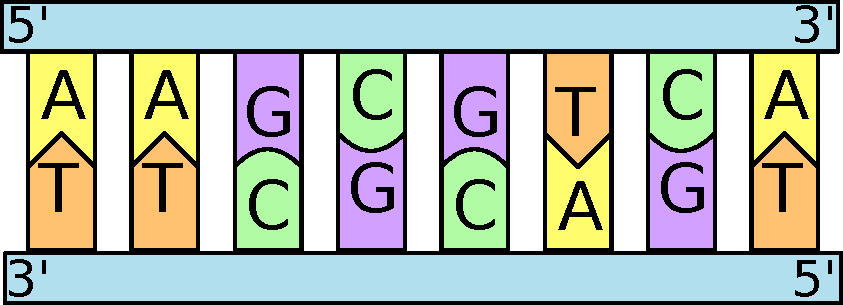
\includegraphics[scale=0.5]{dna-strand}
                \caption[Rappresentazione del DNA]{Rappresentazione grafica degli strand che compongono il DNA.}
                \label{fig:dna-strand}
        \end{centering}
\end{wrapfigure}

Oltre questa considerazione, bisogna tenere conto che
l'informazione presente nel DNA
è la stessa a parità di estremità, ma in ordine inverso e
complementato (vedi figura \ref{fig:dna-strand}) (sostituendo
la citosina con la guanina e
l'adedina con la timina). Nel caso di RNA la timina
si sostituisce l'uracile, ma il processo di formazione del RNA
prevede anch'egli questa operazione di complementazione
della sequenza.

Ergo, quando si considera una sequenza (nel caso
dell'assemblaggio del DNA), è necessario tenere presente
che un collegamento fra due sequenze potrebbe considerare
una sequenza posta sullo strand (una delle estremità
che compone l'elica del DNA) opposto e di conseguenza una loro
sovrapposizione potrebbe richiede un preprocessamento della
stringa che la porti ad essere coerente con l'altra, operazione
che prende il nome di \emph{reverse and complement}.

% GFA1
\section{Linee GFA1}
GFA1 è la versione della specifica, essa si concentra nella descrizione
delle sequenze, collegate tra loro da una relazione di \emph{contenimento}
o di \emph{successione}.